\documentclass[a4paper,UTF8]{ctexart}

\usepackage{amsmath, amsthm, amssymb, amsfonts, hyperref, mathrsfs}%美国数学学会的包+?
\usepackage{geometry} %控制界面
\usepackage{bookmark}
\usepackage{fancyhdr} % header & footer
\usepackage{appendix} % 附录
\usepackage{tikz} %作图
\usepackage{graphicx} %插入图片的宏包
\usepackage{float} %设置图片浮动位置的宏包
\usepackage{subfigure} %插入多图时用子图显示的宏包
\usepackage{listings} %引用代码
\usepackage{physics,mathtools} %物理数学工具
\usepackage{comment}
\usepackage{framed}
\geometry{top=2.5cm,bottom=2.5cm,left=2.5cm,right=2.5cm} % 布局要求
\pagestyle{fancy} % fancy分格
\fancyhf{} % 清除所有页眉页脚
\renewcommand\headrulewidth{0.6pt}
\renewcommand\footrulewidth{0.6pt}
\lhead{何金铭 PB21020660$\mid$座位号:2}
\chead{$\beta$吸收1实验数据处理}
\rhead{\thepage}
\lfoot{2023.4.3}
\rfoot{USTC}
%\bibliographystyle{plain} % 引用样式
\everymath{\displaystyle} % display
%============================================================

\begin{document}

\begin{center}
    \textbf{\Large $\beta$吸收1实验数据处理}
    \par \text{\large 何金铭 PB21020660}
\end{center}

\section{测量G-M计数管的坪曲线}

\begin{table}[H]
    \centering
    \begin{tabular}{|c|c|c|c|c|c|c|c|c|c|c|c|c|}
    \hline
        电压/V & 260 & 270 & 280 & 290 & 300 & 310 & 320 & 330 & 340 & 350 & 360 & 370 \\ \hline
        计数N & 0 & 332 & 4331 & 4207 & 4406 & 4160 & 3949 & 4868 & 5006 & 5106 & 5297 & 4910 \\ \hline
        电压/V & 380 & 390 & 400 & 410 & 420 & 430 & 440 & 450 & 460 & 470 & 480 & 490 \\ \hline
        计数N & 5677(5288) & 4491(5140) & 5245 & 5070 & 5444 & 5469 & 5588 & 5533 & 5648 & 5522 & 5538 & 5581 \\ \hline
    \end{tabular}
    \caption{不同电压下G-M计数值记录表}
\end{table}

{\bfseries{\color{red}{注:}}由于在电压值为380V与390V处认为结果不太符合,可能受涨落影响比较大,所以重新测量了一次,为于“()”中的值}

将上述数据画为坪曲线

\begin{figure}[H]
    \centering
    \begin{minipage}[b]{0.9\textwidth}
        \centering
        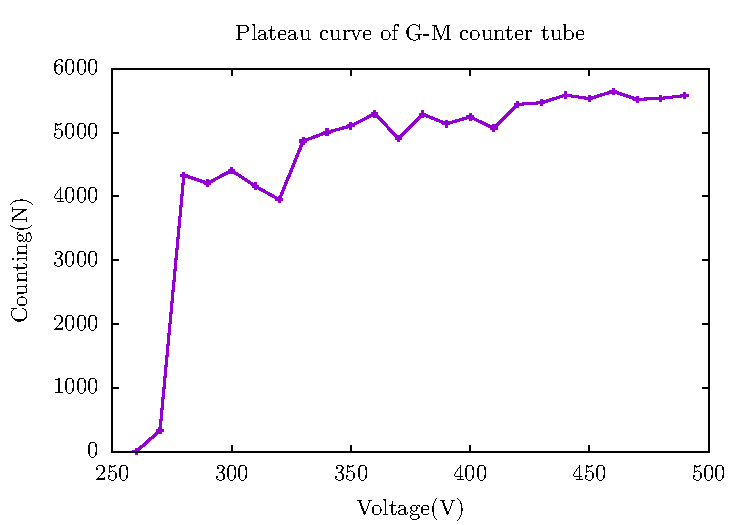
\includegraphics[width=0.9\textwidth]{./fig1.pdf}
        \caption{G-M计数管的坪曲线}
    \end{minipage}
\end{figure}

取刚开始变平缓的电压值为$V_1$,平缓变化快结束的电压值为$V_2$,计算得工作电压为$V = \frac{V_1+V_2}{2} = \frac{230+490}{2} = 360 V$

但由于实验时间的要求,在以下的实验中选用工作电压为430V

\section{测量铝片的质量厚度}

\begin{table}[H]
    \centering
    \begin{tabular}{|c|c|c|c|c|c|}
    \hline
        ~ & 1 & 2 & 3 & 4 & 5 \\ \hline
        m/g & 1.55 & 1.50 & 1.65 & 1.55 & 1.54 \\ \hline
        a/cm & 6.23 & 6.18 & 6.45 & 6.21 & 6.22 \\ \hline
        b/cm & 4.98 & 5.00 & 5.09 & 5.10 & 4.94 \\ \hline
        质量厚度$g/cm^2$ & 0.04996 & 0.04854 & 0.05026 & 0.04894 & 0.05012 \\ \hline
    \end{tabular}
    \caption{GM记录表}
\end{table}

计算得平均质量厚度为$0.04956 g/cm^2$

\section{测量铝片对$\beta$射线的吸收曲线}

{\bfseries{\color{red}{注:}}以下测量均放入了准直孔}

\begin{table}[H]
    \centering
    \begin{tabular}{|c|c|c|c|c|c|c|c|c|c|c|c|c|}
    \hline
        铝片数 & 0 & 1 & 2 & 3 & 4 & 5 & 6 & 7 & 8 & 9 & 10 & 11 \\ \hline
        计数N & 4200 & 3301 & 2575 & 3220 & 2613 & 2124 & 1785 & 1289 & 1270 & 1176 & 1292 & 1274 \\ \hline
        时间/s & 30 & 30 & 30 & 40 & 40 & 40 & 40 & 40 & 50 & 60 & 80 & 100 \\ \hline
        强度$I/s^{-1}$ & 140 & 110.03 & 85.83 & 80.5 & 65.325 & 53.1 & 44.625 & 32.225 & 25.4 & 19.6 & 16.15 & 12.74 \\ \hline
        铝片数 & 12 & 13 & 14 & 15 & 16 & 17 & 18 & ~ & ~ & ~ & ~ & ~ \\ \hline
        计数N & 1122 & 766 & 719 & 641 & 645 & 632 & 648 & ~ & ~ & ~ & ~ & ~ \\ \hline
        时间/s & 120 & 120 & 150 & 200 & 320 & 440 & 760 & ~ & ~ & ~ & ~ & ~ \\ \hline
        强度$I/s^{-1}$ & 9.35 & 6.38 & 4.79 & 3.205 & 2.02 & 1.44 & 0.85 & ~ & ~ & ~ & ~ & ~ \\ \hline
    \end{tabular}
    \caption{GM记录表}
\end{table}

{\bfseries{本底测量时间300s,计数为53}}

计算得本底强度为:$I' = \frac{53}{300} = 0.177$。对上表中的强度进行修正得:

\begin{table}[H]
    \centering
    \begin{tabular}{|c|c|c|c|c|c|c|c|c|c|c|c|c|}
    \hline
        铝片数 & 0 & 1 & 2 & 3 & 4 & 5 & 6 & 7 & 8 & 9 & 10 & 11 \\ \hline
        强度$I/s^{-1}$ & 140 & 110.03 & 85.83 & 80.5 & 65.325 & 53.1 & 44.625 & 32.225 & 25.4 & 19.6 & 16.15 & 12.74 \\ \hline
        铝片数 & 12 & 13 & 14 & 15 & 16 & 17 & 18 & ~ & ~ & ~ & ~ & ~ \\ \hline
        强度$I/s^{-1}$ & 9.35 & 6.38 & 4.79 & 3.205 & 2.02 & 1.44 & 0.85 & ~ & ~ & ~ & ~ & ~ \\ \hline
    \end{tabular}
    \caption{GM记录表}
\end{table}

\begin{figure}[H]
    \centering
    \begin{minipage}[b]{0.9\textwidth}
        \centering
        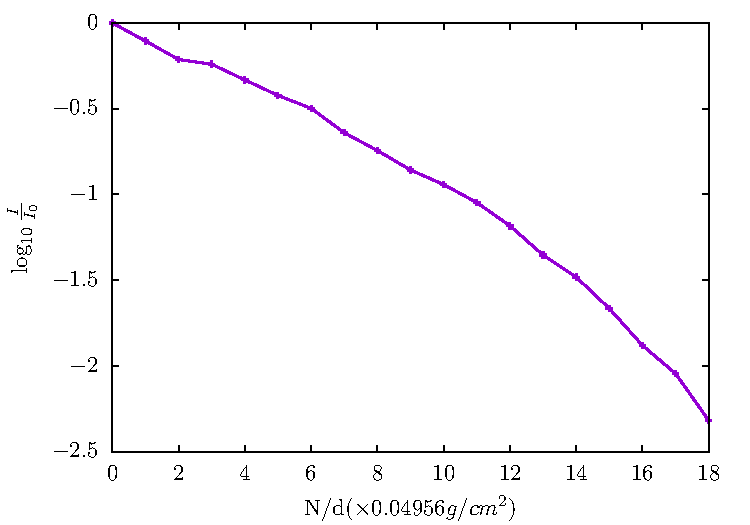
\includegraphics[width=0.9\textwidth]{./fig2.pdf}
        \caption{$\log_{10}{\frac{I}{I_0}}$-质量厚度图}
    \end{minipage}
\end{figure}

拟合曲线为:

\begin{equation}
    \log_{10}{\frac{I}{I_0}} = -0.1213 d + 0.1461
\end{equation}

用前四个点计算得:$h = 0.0504$

用最后4个点计算得:$g(x) = -4.2848 x + 1.5273$

联立后可以解得:$R = \frac{4+1.5273+0.05}{4.2848} = 1.30 g/cm^2$

最终解得:$E = 1.85 \times R + 0.245 = 2.65 MeV$

\end{document}